\part{Introduction}

An embedded system is a combination of hardware and software components put together to achieve a specific task. Often, embedded systems are built into a larger device or system and are used to collect, store, process, and analyse data, as well as to control the device\textquotesingle s behaviour. Embedded devices are a category of tiny devices with physical, computational and memory constraints that are programmable to perform dedicated tasks.

Like most of the automotive industry, Scania employs embedded systems called Electronic Control Units (ECUs) in their trucks to supervise and regulate essential subsystems like the engine, transmission, braking, and electrical systems. Each of these subsystems has one or more ECUs to gather system data and transmit it to a central communicator where the data is processed and the systems operations are monitored.

Scania currently runs a massive fleet of around 600,000 connected heavy vehicles. The company's truck sales make up 62\% of its global sales and Scania has been adding 60,000 trucks to it's fleet annually \cite{scania-report}. This large fleet of rolling vehicles that are connected though the communicators opens up new possibilities. These connected devices continuously monitor the state of the vehicle and this data can be used to accurately
and efficiently schedule vehicle maintainance. For example, if a tire change is predicted to be required in 100 kms then the driver can plan the route smartly to reach the workshop before the vehicle breaks down. This opportunity can be realised by running smart algorithms on the hardware that is currently available.

Machine learning (ML) on embedded devices is becoming increasingly popular due to its ability to provide real-time insight and intelligence to devices. This technology can be used to automate tasks, improve efficiency, and make better decisions. But this technology presents a unique set of challenges due to the limited resources available on these devices. Embedded devices are designed to be power efficient, have limited memory and processing power, and require closely tailored algorithms, making it difficult to use pre-existing machine learning models. Furthermore, embedded devices are often expected to produce real-time results, which further complicates the development process. Despite these challenges, machine learning on embedded devices has potential applications in a variety of areas, such as in the fields of robotics and autonomous vehicles.

One such ML application Scania has been developing in their \textsc{LOBSTR} \cite{lobstr} and \textsc{FAMOUS} \cite{famous} projects is anomaly and fault detection on the vehicles. Targeting to run the anomaly detection models on the existing ECUs with limited resources has many benefits and challenges.

\subsection*{Benefits to performing Anomaly Detection on ECUs}

\begin{itemize}
	\item Scania is committed to promote a shift towards autonomous and eco-friendly transport systems. The latest addition of Scania's connected trucks and buses will be embedded with upgraded ECUs and communication devices. However, this upgrade will make the stock of older hardware devices to become obsolete and regarded as e-waste, which could be prevented. Exploring the possibility of repurposing existing ECUs to run ML models aligns with Scania's vision of leading the way towards a sustainable future.
	\item Neural networks (NNs) are a type of machine learning that can detect intricate patterns not only across multiple data signals but also over time. \textit{include benefits to NN approach to Anomaly Detection}
	%Achieving this level of performance is computationally demanding, and training NNs on embedded devices requires careful resource management. However, being able to efficiently train NNs on embedded devices with high accuracy could unlock significant potential for future advancements. (could include benefits of NN for anomaly detection)
	\item Federated learning methods facilitate the training of pre-trained anomaly detection models on the ECUs installed in Scania's distributed fleet of connected trucks. Each ECU individually trains the model with its data and transmits the updated model parameters to a central server. This distributed learning approach enables early detection of faults or failures and ensures that critical data remains on the device. Also dependency on network bandwidth is reduced as only the aggregated model updates are communicated over the network, instead of transmitting the entire data sample.
\end{itemize}

\subsection*{Challenges to implementing Federated Models}

\begin{itemize}
	\item To reap the best benefits of these approaches, training of the model needs to be performed on board. However much of the potential of running machine learning applications on these devices remains unattained due to the difficulties in creating these applications and running training on-board. Approaches such as TensorFlow Lite (TFLite), Edge Impulse, and STM Cube AI implemented along the TinyML frameworks, enable running ML models targeted for small resource devices. However these approaches are largely limited to inference capabilities and there is no adequate open source support in the existing infrastructure for training ML models.
	\item An Original Equipment Manufacturer (OEM) is responsible for the development and upkeep of the Scania ECU. However, the amount of information made available regarding the hardware design, memory layout, and operating system (OS) is restricted. To construct an embedded OS for a customized hardware, critical details such as the device tree, memory organisation, and boot flow are necessary. Obtaining this information from a functional board can be an enormous task requiring reverse engineering expertise.
\end{itemize}

% Gap in the market: No support for training ML models on embedded devices ❓

% TODO: Attach a reference for the following claim (Ask Niklas)

% Among the ML approaches to take, Artifical Neural Networks are especially interesting for anomaly detection due to several factors such as minimal data preprocessing \dots To get the best out of this approache, training of the model needs to be performed on-board. However much of the potential of running machine learning applications on these devices remain unattained due to the difficulties in creating these applications and running training on-board.

\subsubsection{Problem Description}

The scope of the thesis is to repurpose the existing Scania ECU and explore the challenges of building targeted NN models and training them on repurposed ECU using different approaches and evaluating their performances.

% ============================================
%        Background
% ============================================

\chapter{Background}

Developing and maintaining applications that rely on neural network models and run on a fleet of embedded devices has several considerations. The application deployment process should allow for continuous updates to the neural network, transfer data or model updates from the embedded devices to off-board analytics or machine learnining pipelines, not interfere with the other applications on the embedded device, all the while maintaining correct representations in the neural network model. It is thus important to have an operating system that can support these applications with features such as process isolation, inter process communication mechanisms, multitasking etc.

The target embedded device to run these applications are the ECUs aboard a Scania vehicle. These ECUs have application processor cores that are capable of running rich operating systems such as linux distributions or real-time operating systems such as QNX, or VxWorks. All these operating systems also support hypervisors which allows for configurations where a host operating system runs standard automotive applications in addition to a guest operating system running the neural network application. This approach has the advantage of mitigating application crashes in the guest operating system and can provide a level of protection against software vulnerabilities \cite{linux-guest-os}. Linux is the prefered choice for such a guest operating system due to its configurability and rich support for application development.

The next section looks at developing such an embedded linux environment and the process of developing neural network applications for that operating system.

\section{Development Process for Embedded Linux}

Building and maintaining embedded linux distributions with the linux kernel and user mode applications require tools that can support multi-level build configurations, interface with or build a cross compiling toolchain, support \texttt{C} run times such as glibc or musl, and provide support for project management. There are several tools that provide this support such as OpenADK, The Yocto project, Buildroot, OpenWrt, etc., with The Yocto project and Buildroot being the most featureful and presently the most widely used embedded linux build systems. In comparison with Buildroot, the Yocto project supports a greater variety of hardware and also has faster incremental build times as it caches the generated binaries. The Yocto project was chosen as the primary build system and used to generate the embedded linux and application programs used within this project.

% TODO : Discuss and possibly add reference to https://aaltodoc.aalto.fi/handle/123456789/115155

\subsection{SDKs and Compiler Toolchains}

Creating applications for embedded devices requires a set of software components that are usually collectively referred to as Software Development Kits (SDK). This suite of programs usually contain a toolchain that is capable of converting application source code, such as those in \texttt{C}  or \texttt{C++}, into executables that can be run on the target embedded device.

Software development toolchains consists of a compiler, linker, libraries, debuggers, as well as a collection of programs to create and manage executable binary programs for a target device such as the commonly used GNU binary utilities, a.k.a binutils. The primary choice for a \texttt{C} compiler is the GNU Compiler Collection \texttt{GCC}, with LLVM's Clang being the closest alternative. To develop applications that interface with the linux operating system APIs, the toolchain also contains necessary header files called linux kernel header files. The last important piece of a toolchain will be the \texttt{C} runtime, with the most popular choice being GNU's glibc.

\subsection{Cross Compiling and Application Development}

The software development toolchains for embedded devices are generally run on a development machine that is different from the embedded device. In this configuration the compiler toolchain creates executables for a different platform that the one it is currently running on and is termed a cross compiling toolchain. A compiler toolchain that creates executables for the sample platform is termed a native compiler toolchain. Cross compilers are common due to several factors such as limited resources on embedded devices, ease of targetting multiple hardware platforms, and ultimately is unavoidable as someone somewhere has to do some amount of cross compiling in order to create programs for a new hardware platform. Most software that are run on embedded devices are created on different computing hardware devices usually termed development hosts.

\begin{figure}[h]
	\centering
	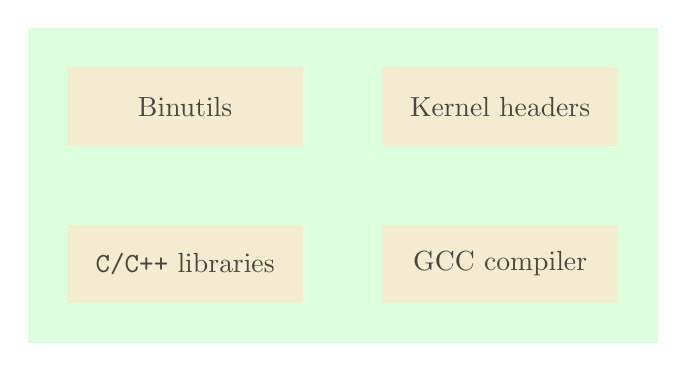
\begin{tikzpicture}[fill opacity=0.7]
		\fill[green!20] (0.5,0.5) rectangle (8.5, 4.5);
		\fill[orange!20] (1,3) rectangle (4, 4);
		\draw (2.5, 3.5) node {Binutils};
		\fill[orange!20] (5,3) rectangle (8, 4);
		\draw (6.5, 3.5) node {Kernel headers};
		\fill[orange!20] (1,1) rectangle (4, 2);
		\draw (2.5, 1.5) node {\texttt{C/C++} libraries};
		\fill[orange!20] (5,1) rectangle (8, 2);
		\draw (6.5, 1.5) node {GCC compiler};
	\end{tikzpicture}
	\caption[toolchains]{Primary components of a \texttt{GCC} based cross compiling toolchain for embedded linux.}
\end{figure}

Another common alternative to cross compiling in this manner is by using native compilers via emulation. Emulation is some technique that allows a computer system usually termed host to simulate the behaviour of some other computer system usually termed guest. There are several software projects that allow for emulation in this manner with QEMU being by far the most commonly used emulator targetting several different hardware platforms. QEMU can also be used to test the applications created via this process before being deployed on the target hardware. Application development for embedded devices usually employs cross compiling toolchains and emulation software to create, test, and maintain the software.

\subsection{Target Device}

Building an embedded linux kernel suited for a mainboard of an embedded device requires appropriate build configurations describing the kernel, its enabled feature, the device tree layout, i/o memory mapping, etc \cite{bootlin-port}. These parameters are a description of the devices on the mainboard, their interfaces to the processor, and the nature of the embedded linux that is to be managing the hardware platform. To port linux onto a processor on a particular board requires creating a boot loader capable of that task as well. A boot loader program is responsible for placing an operating system into memory. This process will also need software and configurations that need to be supported by the build configurations that the embedded linux build system will use. The majority of the details as to how the boot loader has to be configured will be based on the particulars of the hardware that it will be configured for.

The initial target machine was an ECU filling the role of a communicator on the truck. Certain support components for this board are unavailable, such as the Yocto meta layer used for the existing software on board, memory mapping for the attached devices, source codes for boot ROM firmware or the boot loader, etc. The reverse engineering efforts to attain this information were dropped due to time constraints and ultimately a similiar board, namely the iMX6SDB evaluation board, with the required information publicly provided by processor chip vendor NXP was chosen as the target platform. The details of the attempt at uncovering this information is layed out in \hyperref[rtc-c300]{Appendix II}.

\section{Neural Network Application Development}

The most popular ways to write neural network models are by using machine learning frameworks such as Tensorflow, MXNet, PyTorch, Caffe, etc. These machine learning frameworks themselves are build on top of multiple software libraries meant for specific aspects of performing machine learning calculations. For instance, a neural network model described in Python using Keras gets converted to a computational graph representation in Tensorflow. Then depending on the model, its invocation, and the compute platform its running on, Tensorflow may use other software libraries such as XNNPACK, or Intel oneAPI Math Kernel Library to perform the calculations. Several libraries exist that target specific subproblems in such computations and provide optimised implementations of several different processor architectures.

\subsection{Choice of Software Stacks and Programming Languages}

As most neural network applications are written in frameworks like PyTorch and Tensorflow, they have thriving ecosystems that provide rich developer support. Most neural network models are trained in a rich compute environments with either dedicated machine leanring computer systems or general purpose computer systems with plentiful operational capacities. Machine learning based companies and their service offerings such as cloud machine learning platforms almost invariably targets these platforms and provide several software tools for developers to utilize. Developers in these platforms enjoy several resources such as productivity tools that allows for continuous integration and development, maintainance and other resources with features for performance profiling, debugging, orchestration, etc.

% TODO : Consider examples from https://github.com/EthicalML/awesome-production-machine-learning

The programming environment for embedded devices however are not as featureful or supported as those mentioned previously. Developer resources such as productivity tools for neural network application development and maintainance are lacking and the software stacks that are traditionally used are either too large or unsupported on the broader embedded hardware platforms.

Another aspect to consider is the programming language and software stack used to describe a neural network application. Most machine learning models at present are written in Python and frameworks like PyTorch and Tensorflow have richer interfaces for Python compared to other programming languages. This may be unfavourable to embedded devices where a Python application may take up higher memory and have longer latencies. The programming language of choice for embedded applications is \texttt{C} and \texttt{C++} which are supported by the ML frameworks but not to the same extent as their Python interfaces.

\subsection{Embedded Software Stacks for Neural Networks}

One complication caused by relying on software stack of the manner discribed before is software bloat. This causes a bigger problem in the context of embedded devices where resources are limited. There has been significant efforts made to clear this concern for the world of embedded devices \cite{tinyml}, especially motivated by interests in getting neural network applications ready for mobile devices \cite{tfl} \cite{pytorch-mobile}

\section{Training on Device}

The traditional model for developing machine learning applications on embedded devices has several discrete steps such as collecting sensor data from the embedded devices

\subsection{Federated Learning}

Federated learning is a technique of training ML models in a distributed way, where each client or device uses its own data set to train a local model. A client application on a truck generates sensor data created by the operation of the vehicle. Each vehicle then trains on-board a local model which is then centrally collected and aggregated to build a global model. This global model can then be used for inference in each client. In the LOBSTR \cite{lobstr} and FAMOUS \cite{famous} projects Scania has developed statistical models and NN models for anomaly detection. The statistical models are lightweight and can easily be trained with limited computational resources. These neural network models are computationally heavy and hard to train with limited resources. The existing ECUs are not tailored for ML and general purpose ML frameworks often are hard to use in this embedded systems, specially for training purposes.

This thesis focuses on repurposing existing hardwared (ECU) to ML edge devices that are tailored to train NN in the most efficient possible way. We try to reverse engineer the old communicator model to build a custom Yocto project tailored for ML. As alternative test ECU we use an evaluation board that has similar specifications as the commuicator to benchamark and experiment different NN implementations and evauluate the optimal ones.


% ============================================
%        Theory
% ============================================

\chapter{Theory}

The first section in this chapter lays out an overview of the training process of neural networks. The following section introduces some terminology associated with software development for embedded devices, contextualised in embedded linux and its application development. The final section gives a short overview of conducting application performance evaluation.

\section{Neural Network Training}

In terms of the calculations performed by a computer system, training a neural network model reduces to performing several multiplication and addition operations on floating point values. To motivate this point of view, consider the following account of neural network models and their training process.

\section{Embedded Linux Environment}

As presented in the preivous chapter, the development, deployment, and maintainance of embedded linux distributions and their user mode applications are usually managed using capable build systems. Configuring these systems requires understanding concepts such as boot sequence, file system interfaces, boot loaders, root filesystems, cross compiling toolchains (introduced in the preceding chapter), etc.

\subsection{A Simplified Embedded Boot Sequence}


\begin{figure}[h]
	\centering
	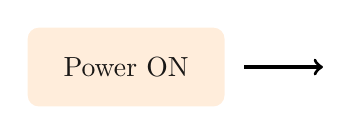
\begin{tikzpicture}[fill, rounded corners, opacity=0.7]
		\fill [orange!20] (0,0) rectangle (2.5, 1);
		\draw [opacity=0.9] (1.25, 0.5) node {Power ON};
		\draw [->, very thick, opacity=1] (2.75, 0.5) -- (3.75, 0.5);
	\end{tikzpicture}
	\caption[boot-sequence]{A simplified embedded linux boot sequence.}
\end{figure}

\section{Performance Evaluation}



Roofline model for a simple matrix multiply application on Cortex-A9
